\documentclass[10pt,twocolumn]{article}
\usepackage[margin=0.6in]{geometry}
\usepackage{graphicx}
\usepackage{booktabs}
\usepackage{amsmath}
\usepackage[dvipsnames]{xcolor}
\usepackage{titlesec}
\usepackage[font=footnotesize,labelfont=bf]{caption}
\usepackage{lmodern}
\usepackage{microtype}
\usepackage{stfloats}
\usepackage{enumitem}
\usepackage{listings}
% AUTO-GENERATED by this snippet from figures/*.json -- do not hand-edit
\newcommand{\tablerandom}{%
\begin{tabular}{lccccc}
\toprule
method & $m{=}1$ & $m{=}3$ & $m{=}5$ & $m{=}10$ & $m{=}20$ \\
\midrule
sample score & 0.457 & 0.241 & 0.184 & 0.132 & 0.084 \\
CAPA kNN & 0.399 & 0.260 & 0.181 & 0.121 & 0.069 \\
2PL IRT & 0.129 & 0.098 & 0.080 & 0.067 & 0.046 \\
raw-trace blend & 0.098 & 0.083 & 0.072 & 0.063 & 0.044 \\
qubric geometry & 0.091 & 0.072 & 0.067 & 0.062 & 0.060 \\
\textbf{qubric blend} & \textbf{0.090} & \textbf{0.068} & \textbf{0.059} & \textbf{0.051} & \textbf{0.039} \\
\midrule
$\Delta$(blend $-$ IRT) & -0.039 {\scriptsize [-0.050,\,-0.028]} & -0.030 {\scriptsize [-0.037,\,-0.023]} & -0.021 {\scriptsize [-0.026,\,-0.015]} & -0.015 {\scriptsize [-0.019,\,-0.011]} & -0.006 {\scriptsize [-0.009,\,-0.004]} \\
\bottomrule
\end{tabular}}

\newcommand{\tableadaptive}{%
\begin{tabular}{lccccc}
\toprule
method & $m{=}1$ & $m{=}3$ & $m{=}5$ & $m{=}10$ & $m{=}20$ \\
\midrule
adaptive 2PL IRT & 0.077 & 0.062 & 0.053 & 0.040 & 0.032 \\
raw-trace blend & 0.074 & 0.058 & 0.051 & 0.038 & 0.032 \\
qubric geometry & 0.074 & 0.068 & 0.064 & 0.060 & 0.055 \\
\textbf{qubric blend} & \textbf{0.066} & \textbf{0.053} & \textbf{0.047} & \textbf{0.040} & \textbf{0.032} \\
\midrule
$\Delta$(blend $-$ IRT) & -0.011 {\scriptsize [-0.019,\,-0.003]} & -0.009 {\scriptsize [-0.015,\,-0.002]} & -0.006 {\scriptsize [-0.013,\,+0.001]} & +0.000 {\scriptsize [-0.005,\,+0.006]} & -0.000 {\scriptsize [-0.005,\,+0.004]} \\
\bottomrule
\end{tabular}}


\definecolor{ink}{HTML}{0A1638}
\definecolor{navy}{HTML}{2E5CA6}
\definecolor{amber}{HTML}{D97706}
\titleformat*{\section}{\large\bfseries\color{ink}}
\titleformat*{\subsection}{\normalsize\bfseries\color{ink}}
\setlength{\parskip}{2pt}
\renewcommand{\topfraction}{0.95}
\renewcommand{\dbltopfraction}{0.95}
\renewcommand{\textfraction}{0.05}
\renewcommand{\dblfloatpagefraction}{0.90}
\setcounter{dbltopnumber}{3}
\lstset{basicstyle=\ttfamily\scriptsize,breaklines=true,frame=single,
  rulecolor=\color{ink!25},backgroundcolor=\color{ink!4},framesep=4pt,
  aboveskip=4pt,belowskip=4pt,columns=fullflexible,keepspaces=true}

\title{\vspace{-1.2em}\textbf{Embedding agentic traces for efficient evaluation}}
\author{Helivan \quad Jataware \quad Johns Hopkins}
\date{Summer 2026}

\begin{document}
\maketitle

\section*{The problem}
Evaluating an agentic system is expensive: one SWE-bench Verified entry is
500 agent executions at \$0.13--\$4 per instance (HAL's measured aggregate:
\$1.84 per rollout), so each model checkpoint, scaffold tweak, and
configuration variant costs on the order of \$100--\$2{,}000 and hours of
wall-clock to score. Meanwhile the runs already performed by others sit in
public archives: trajectories and outcomes for 100+ systems. We ask how
accurately a \emph{new} system's full-benchmark score can be predicted from
a handful of probe runs, using that cache as reference.

Correctness-only approaches (IRT, adaptive testing, score-matrix
compression) extract at most a few bits per probe. But each probe also
produces a \emph{trace} --- a tool-call log of $10^4$--$10^5$ tokens
recording how the system worked --- which carries far more information
than its pass/fail bit. The obstacle is that off-the-shelf trace
embeddings are dominated by \emph{confounders}: nearest neighbors are
same-system 68--83\% of the time, same-scaffold at $5\times$ chance, and
the exact configuration is identifiable at twice chance even among
same-model, same-harness siblings --- while agreement with outcome sits at
chance.

\section*{What efficient evaluation requires of an embedding}
Reference-based prediction compares the new system's probe traces against
cached traces of systems with known scores. This breaks in a specific way
when the embedding matches on \emph{who built the system} rather than
\emph{what it did}: prediction degenerates into copying scores from the
target's LLM-family or harness siblings --- accurate-looking under naive
cross-validation (we measure $\sim$25\% inflation), and wrong exactly when
it matters, for systems without siblings in the cache. \textbf{For
efficient evaluation, an embedding should not rely on confounders --- LLM
family, harness, configuration identity --- and should instead rely on
content.} Concretely:
\begin{itemize}[leftmargin=1.2em,itemsep=1pt,topsep=1pt]
  \item \textbf{content-faithful}: traces of different systems on the same
  task, doing similar work, should embed similarly (task and behavioral
  fidelity);
  \item \textbf{confounder-invariant}: harness, model family, and exact
  configuration should be near chance-level recoverable;
  \item \textbf{stable}: the same trace, re-processed, should map to
  approximately the same place (the pipeline's stochastic stages are
  rubric creation and extraction).
\end{itemize}
Each requirement is measurable, and the confounder requirement is also
enforced in evaluation by a conservative protocol: references sharing the
target's underlying LLM are excluded (leave-one-LLM-out; robustness under
leave-one-harness-out is verified separately).

\section*{qubric}
Our method for embedding agentic traces is based on a query-specific
rubric. For each task instance an LLM (Model~1) reads the public problem
statement and writes a query-specific rubric comprised of
1)~understanding, 2)~localization, 3)~reproduction, 4)~editing,
5)~verification, and 6)~final state. Given a trace corresponding to the
task, a judge LLM (Model~2) extracts a short factual description per
section. The short descriptions are then embedded with an off-the-shelf
embedding model, centered against the cross-system median per instance,
and concatenated. This approach enforces the equivalence relations the
space should respect by respecting the rubric and using a fixed judge LLM
as the extractor. (Configuration for all results: Model~1 = Model~2 =
DeepSeek-V4-Flash-0731 reading full pruned traces; embedder
text-embedding-3-small; 107 systems $\times$ 100 tasks; total pipeline
cost $\approx$\$26.)

\begin{figure*}[t]
  \vspace{-6pt}\centering
  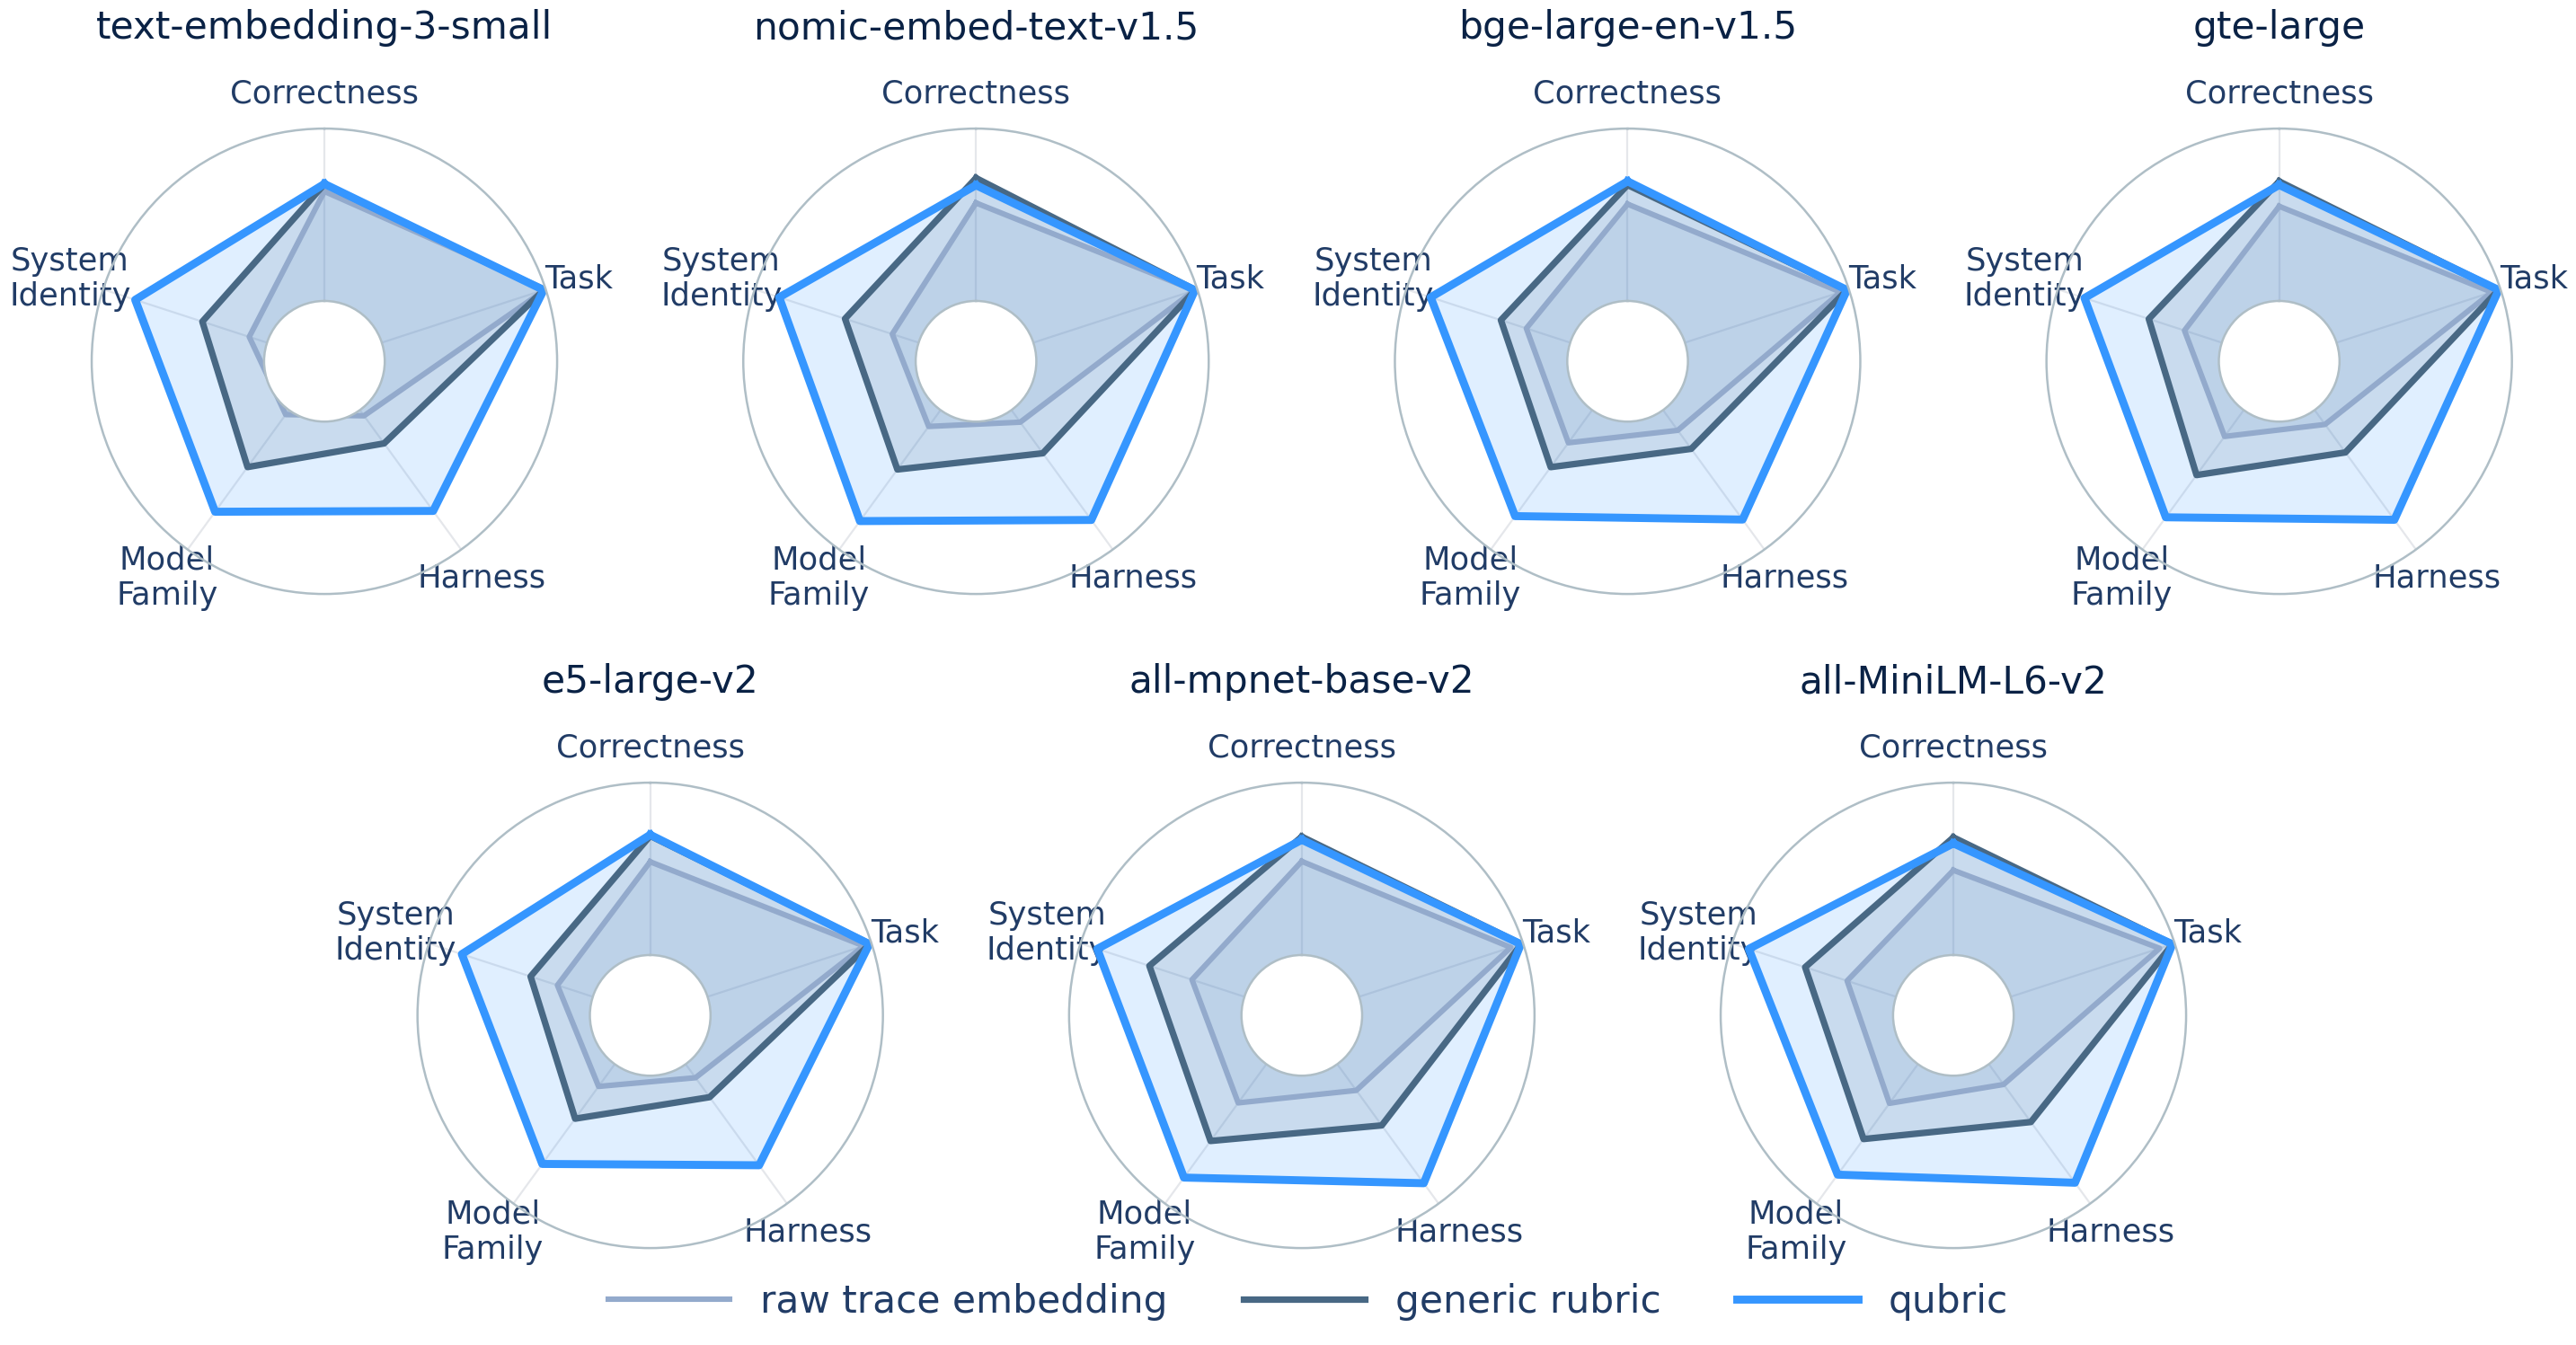
\includegraphics[width=\textwidth]{../figures/radar_all.png}
  \caption{Qubric has the sensitivity profile efficient evaluation
  requires, across seven embedders (rim = ideal). Raw embeddings (navy)
  are confounder-dominated; qubric (amber) collapses Identity / Model
  family / Harness to chance while holding Task and Behavior.}
  \label{fig:radar}
\end{figure*}

\section*{Qubric meets the requirements; raw embeddings do not}
Across seven embedding models, qubric collapses the confounder axes to
approximately chance (harness $0.31\!\to\!0.08$, model family
$0.20\!\to\!0.12$, identity $0.83\!\to\!0.09$) while retaining task
fidelity ($\sim$0.95; Figs.~\ref{fig:radar},~\ref{fig:heatmap}). The
confounder-reliance of raw embeddings is visible directly in the
evaluation curves below: raw-trace prediction error is \emph{flat} in the
number of probes ($0.100\!\to\!0.093$ MAE from 1 to 20 probes) ---
additional raw traces mostly re-measure who the system is --- while
qubric keeps improving ($0.091\!\to\!0.060$). Stability is measured, not
assumed: the same trace re-processed retrieves its first-pass twin at
trace level $0.32$; system-level positions recover to $0.80$ after
aggregating 20 instances, and rewriting the rubric costs only a further
$0.03$.

\begin{figure}[t]
  \centering
  \includegraphics[width=\columnwidth]{../figures/independence_heatmap.png}
  \caption{Requirements by representation: each cell is the raw metric for
  that axis under that representation; blue = ideal for evaluation. Qubric
  is the only row simultaneously content-faithful and
  confounder-invariant.}
  \label{fig:heatmap}
\end{figure}

\section*{Efficient evaluation results}
A new system runs $m$ probes; we predict its full 500-instance resolve
rate. The trace channel (qubric geometry: product-kernel PKPS comparison
against references' full cached coverage; bandwidth and $k$
cross-validated on references) is blended with the strongest
correctness-only channel (2PL IRT; adaptive item selection where probes
are chosen) via a reference-selected weight $\alpha$. All results are
leave-one-LLM-out over 107 systems; 95\% bootstrap CIs over systems;
paired deltas test the trace contribution.

\begin{table}[t]
\centering\scriptsize
\resizebox{\columnwidth}{!}{\tablerandom}
\caption{Random probes (B=20 draws): MAE predicting the true resolve
rate. The blend beats the best correctness-only method at every budget;
all paired deltas exclude zero.}
\label{tab:random}
\end{table}

\begin{table}[t]
\centering\scriptsize
\resizebox{\columnwidth}{!}{\tableadaptive}
\caption{Adaptive probes (per-target CAT panels). The blend is
best-or-tied everywhere; the trace increment is significant at $m\le3$
and vanishes as correctness information saturates ($m\ge10$).}
\label{tab:adaptive}
\end{table}

Three structural findings. (1)~\emph{Traces matter most when probes are
scarce}: the paired trace increment is largest at $m{=}1$ ($-0.039$,
random regime) and decays monotonically; the blend weight $\alpha$ rises
with $m$ accordingly. (2)~\emph{The judge stage earns its cost}:
replacing qubric with raw-trace embeddings inside the identical blend
loses 0.004--0.008 MAE at $m\le5$ in every regime. (3)~\emph{Predictions
do not lean on siblings}: swapping the held-out sibling axis from LLM to
harness moves the blend by at most 0.004.

\begin{figure}[t]
  \centering
  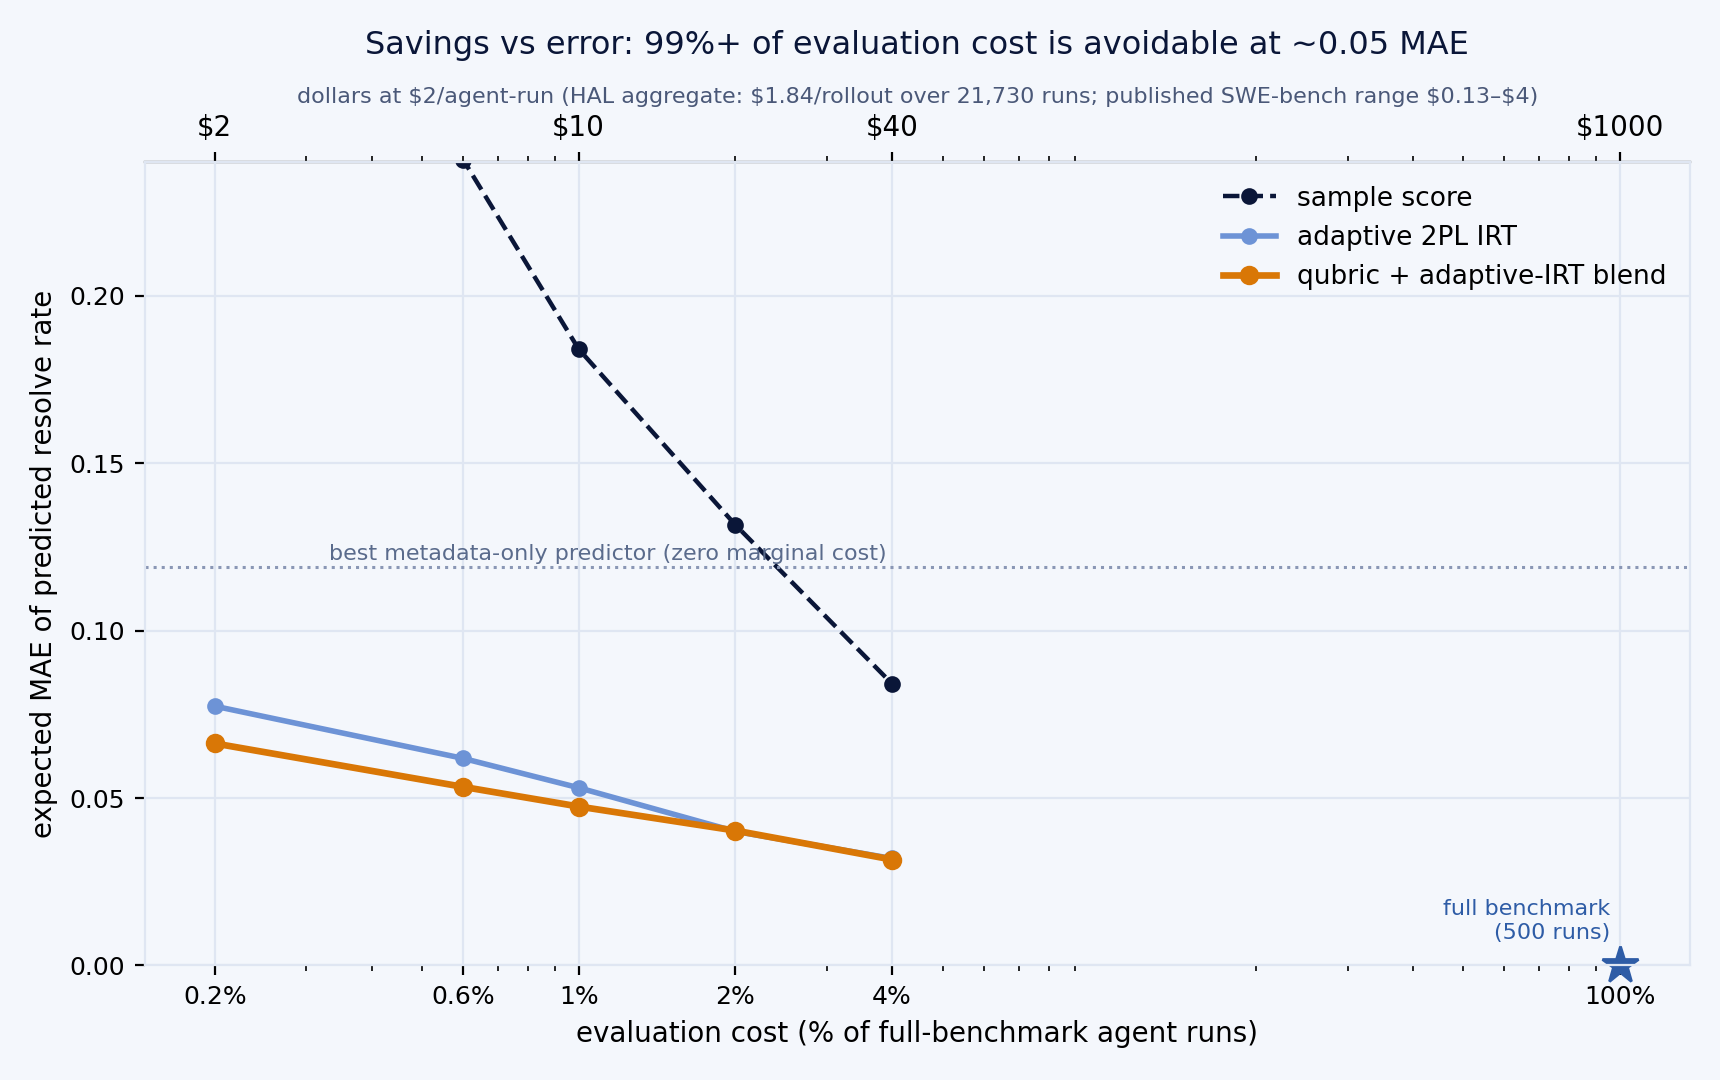
\includegraphics[width=\columnwidth]{../figures/fig_savings.png}
  \caption{Savings vs.\ error. At 1\% of full-benchmark cost ($\sim$\$10
  at HAL's measured \$1.84/rollout average) the blend predicts the final
  score within $\sim$0.048; at 4\% ($\sim$\$40), within $\sim$0.032.}
  \label{fig:savings}
\end{figure}

The economics (Fig.~\ref{fig:savings}): one probe run ($\sim$\$2) yields a
prediction within 0.066 MAE --- versus 0.457 for that probe's score alone
and 0.119 for the best metadata-only predictor. The one-time cost of
constructing the reference geometry from the public archive was
$\approx$\$26 --- mining roughly \$50K--100K of embodied agent compute
contributed by leaderboard submitters.

\section*{Remaining tasks}
\begin{enumerate}[leftmargin=1.4em,itemsep=1pt,topsep=1pt]
  \item Sensitivity to the choice of Model~1 and Model~2 under the current
  configuration (judge robustness was mapped in the prior configuration;
  rerun at q100).
  \item An additional benchmark, ideally Terminal-Bench (142 systems, 89
  tasks, $\geq$5 trials per task, public trajectories).
  \item A descriptive figure: trace anatomy and the qubric pipeline.
  \item Literature review.
  \item Another downstream task? (Routing? Just needs to beat using the
  off-the-shelf embedding for this paper.)
\end{enumerate}

\onecolumn
\section*{Appendix: a worked example (\texttt{sympy\_\_sympy-14248})}

\subsection*{A. Example trace (excerpt)}
The opening and closing of a sweagent + GPT-4 trace on this instance. Note
how much of the text is harness syntax, state dumps, and format echoes
rather than content; this particular run ends unsuccessfully at the cost
limit.

\begin{lstlisting}
swe_main
First, I'll create a new Python script to reproduce the issue as described. This script will contain the code provided in the issue text. Let's start by creating a file named `reproduce_issue.py`.

action: create reproduce_issue.py

[File: /sympy__sympy/reproduce_issue.py (1 lines total)]
1:

First, I'll create a new Python script to reproduce the issue as described. [...]

action: edit 1:1
from sympy import *
A = MatrixSymbol('A', 2, 2)
B = MatrixSymbol('B', 2, 2)
print(A - A*B - B)
pprint(A - A*B - B)
print(latex(A - A*B - B))
end_of_edit

[... ~40K tokens omitted ...]

Your changes have NOT been applied. Please fix your edit command and try again.
You either need to 1) Specify the correct start/end line arguments or 2) Correct your edit code.
DO NOT re-run the same failed edit command. Running it again will lead to the same error.

(Open file: /sympy__sympy/sympy/plotting/plot.py)
(Current directory: /sympy__sympy)
bash-$
primary
role: assistant
Exit due to cost limit
Exit due to cost limit
action: exit_cost
primary
\end{lstlisting}

\subsection*{B. The qubric path: problem $\to$ rubric $\to$ extraction}
The problem statement for this instance (the benchmark task input --- it
describes the symptom only and does not prescribe a fix):

\begin{lstlisting}
The difference of MatrixSymbols prints as a sum with (-1) coefficient
Internally, differences like a-b are represented as the sum of a with `(-1)*b`, but they are supposed to print like a-b. This does not happen with MatrixSymbols. I tried three printers: str, pretty, and latex:
from sympy import *
A = MatrixSymbol('A', 2, 2)
B = MatrixSymbol('B', 2, 2)
print(A - A*B - B)
pprint(A - A*B - B)
latex(A - A*B - B)
Output:
(-1)*B + (-1)*A*B + A
-B + -A*B + A
'-1 B + -1 A B + A'
Based on a [Stack Overflow post](https://stackoverflow.com/q/48826611)
\end{lstlisting}

\noindent The rubric-generation prompt (Model 1), with the problem statement
above substituted for \texttt{\{problem\}}:

\begin{lstlisting}
Here is a repository issue that a software-engineering agent will be asked to fix:

{problem}

Write an instance-specific rubric for judging an agent's trace on THIS issue:
for each section below, one sentence saying what specifically to look for in
this instance (name the likely relevant modules/files/tests if inferable).

Sections: understanding, localization, reproduction, editing, verification, final_state.
Respond with ONLY a JSON object with those keys, each a one-sentence string.
\end{lstlisting}

\noindent The resulting query-specific rubric. None of the named locations
(\texttt{sympy/printing/}, the three printer classes) appear in the problem
statement --- they are inferred:

\begin{lstlisting}
{
 "understanding": "Look for the agent correctly identifying that MatrixSymbol/MatrixExpr subtraction is being canonically represented as Add with negative terms, but the printers should render binary subtraction for matrix expressions just like scalar expressions, likely involving SymPy's printing layer rather than matrix algebra simplification.",
 "localization": "Look for the agent localizing the bug to the SymPy printers for MatrixExpr/MatrixSymbol, especially StrPrinter, PrettyPrinter, and LatexPrinter in files under sympy/printing/ (for example printers.py, str.py, pretty/pretty.py, latex.py) and any MatrixExpr-specific handling that bypasses standard Add printing.",
 "reproduction": "Look for a minimal reproduction using the exact example A = MatrixSymbol('A', 2, 2); B = MatrixSymbol('B', 2, 2); print(A - A*B - B), pprint(...), latex(...), with observed outputs showing '-1' coefficients instead of subtraction, and ideally an added regression test capturing these outputs.",
 "editing": "Look for a focused code change that teaches the relevant printers to display Add terms involving MatrixExpr/MatrixSymbol negatives as subtraction rather than '-1*term' formatting, without changing symbolic semantics or simplification behavior.",
 "verification": "Look for the agent running or reasoning about targeted printer tests in SymPy's test suite - likely tests/printing/test_str.py, test_pretty.py, and test_latex.py or matrix-related printer tests - and confirming the example now prints correctly.",
 "final_state": "Look for the final state to include a passing regression test for matrix subtraction printing, no changes to algebraic canonicalization of MatrixExpr, and correct output for str, pretty, and latex on the provided example."
}
\end{lstlisting}

\noindent The judge (Model 2) reads the full trace through this rubric and
emits one short factual description per section; these six texts are what
gets embedded. Note the honest record of an unfinished trajectory:

\begin{lstlisting}
{
 "understanding": "The agent recognized the bug by reproducing the issue with MatrixSymbol subtraction, noting that outputs showed '-1' coefficients instead of subtraction. It understood the problem was in the printing layer and proceeded to fix it without analyzing canonical representation details.",
 "localization": "The agent localized the bug to SymPy's printing module by searching for MatrixSymbol in files and examining latex.py, focusing on _print_MatrixSymbol and _print_Add methods in printers like StrPrinter, PrettyPrinter, and LatexPrinter.",
 "reproduction": "The agent created a minimal reproduction script with A = MatrixSymbol('A', 2, 2); B = MatrixSymbol('B', 2, 2); and printed str, pretty, and latex outputs, confirming the issue with '-1' coefficients in all printers.",
 "editing": "The agent started editing latex.py by adding a _print_MatrixSymbol method and planned to modify _print_Add, but was diverted to fix deprecation warnings in other files like plot.py, leaving the main edit unfinished and cost limit reached.",
 "verification": "The agent never ran or reasoned about targeted printer tests in the test suite; verification was limited to running the reproduction script, and no tests from tests/printing/ were executed or considered.",
 "final_state": "The final state did not include a passing regression test or completed fix; the agent was still addressing deprecation warnings and had not finalized changes to ensure correct str, pretty, and latex outputs for matrix subtraction."
}
\end{lstlisting}

\end{document}
